% The stage-9 window figure of Section 5 (defined here so that it floats to the page where Section 5 starts)
\begin{figure*}[t]
  \centering
  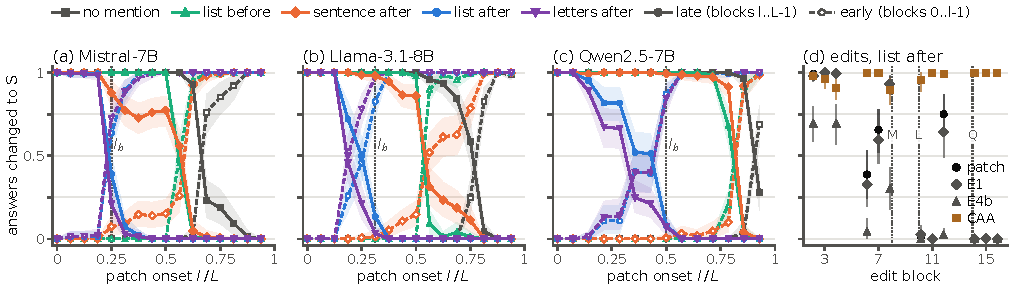
\includegraphics[width=\textwidth]{figures/fig_window.pdf}
  \caption{\textbf{With the candidates listed after the story, a patch of the writing token's cache must reach its early layers to change the answer.} Stage 9. (a--c)~Share of generated answers changed to S, the source story's value, by the late patch (S's key and value at the writing token from block $l$ to the top; solid) and by the early patch (below block $l$; dashed), against the onset $l$ as a fraction of the depth $L$, by format (\NqStories{} new stories; 95\,\% two-stage cluster intervals as bands); dotted: $l_b$, the first onset whose late patch changed at most 0.2 of \fmtListA{} answers on earlier stories. (d)~Share of \fmtListA{} answers changed by edits written at blocks 3--15: the natural patch, single-site steering (E1), the trained remap (E4b; not run at Llama) and steering at every position from the writing token on, generated tokens included (CAA); in each block, Mistral-7B, Llama-3.1-8B and Qwen2.5-7B from left to right; dotted: $l_b$ (M, L, Q: blocks \NqLbMistralSeven, \NqLbLlamaEight, \NqLbQwenSeven; \NqCores{} edit cores).}
  \label{fig:window}
\end{figure*}

\section{A match at the later mention, read by key}\label{sec:claim2}

\textbf{In two 7B models (Qwen2.5-7B, Mistral-7B), the reader heads match the writing token's key at the later mention of the written value and write a flag into that mention's row, which the answer reads by key.} The flag suffices to move the answer but is neither specific nor the only carrier, and the question sets the sign of the read (details in \cref{app:claim2-brief}, \cref{fig:flag}).

\paragraph{Two hops.}
In the discovery sample, 5\,\% of heads, the \emph{reader heads}, read the writing token's key at the option words (hop~1): seeing the clamped key alone, they recover \HoneRQwenSeven{} and \HoneRMistralSeven{} of the option rows' read (\cref{app:heads}). They are enriched for duplicate-token heads \citep{wang2022ioi} (exploratory). Mean-ablating them at the option rows leaves \HthreeRhoQwenSeven{} and \HthreeRhoMistralSeven{} of the key read and raises the value read: a copy route stays available. The answer reads the option words, not the writing token (hop~2), mainly by key, so in lists the written value is read at its later mention, not looked back for at the token that states it.

\paragraph{What the readers write.}
The reader heads write one vector per layer into the re-mentioned word's row. We call it the \emph{flag}. Injected with no key clamp into the row of an option absent from the story, a version fit without that word moves the answer there (\JdOneRatioQwenSeven{} / \JdOneRatioMistralSeven{} of the key read's identity effect; the answer changes in \pct{\JdOnePiXQwenSeven} / \pct{\JdOnePiXMistralSeven} of stories)\rsk; like the natural key clamp, the injection adds the flag at that row and removes it at the base value's row. Its mean direction names no candidate. The answer reads it by key, as it reads the natural one (giving only the answer row the option rows' original keys removes \JdFourKQwenSeven{} / \JdFourKMistralSeven{} of its effect). But the prediction\rsk{} that it is specific failed against structured controls, and one direction per layer does not carry the key read ($\rho_K$ = \JdThreeRhoFlagQwenSeven{} / \JdThreeRhoFlagMistralSeven{}): other carriers exist; the flag is sufficient but not necessary. Removing it leaves about half of the key read, as the prediction\rsk{} allowed, but the line failed on its control directions, which overlap the flag (\cref{app:decisions}). % verbatim: outcome J part D

\paragraph{The sign of the read.}
Asked which option was \emph{not} mentioned, both reads turn negative and the same reader heads carry them; that the sign is applied after the first hop is exploratory. In indirect-object identification (IOI) with the names re-mentioned in a parenthesis, the key read is negative and the value read positive in both models, consistent with S-inhibition \citep{wang2022ioi}, and the negative read is applied where the answer reads the listed names, more by key than by value (restoring their keys and values for the answer row alone removes \JdRouteKVQwenSeven{} / \JdRouteKVMistralSeven{} of it)\rsk. The prediction\rsk{} that the ten answer-side heads ranked in lists apply it failed: a different (or a distributed) reader applies the negative read. That the belief readers carry the IOI read\rsk{} was met at Qwen2.5-7B and is not evaluable at Mistral-7B. The flag is written in sentences as in lists at 1.5B--7B, but four further predictions\rsk{} did not hold: that it carries the size of the sentence read across scale and is read by value at 1.5B (the decision table gives ``Mixed.''), that the initial-state flag carries binding separably from order, and that a key naming no candidate acts as removing the base value's flag (\cref{app:sign,app:scale}).
